\clearpage

\section{Appendix}
\begin{figure}[h!]
  \centering
  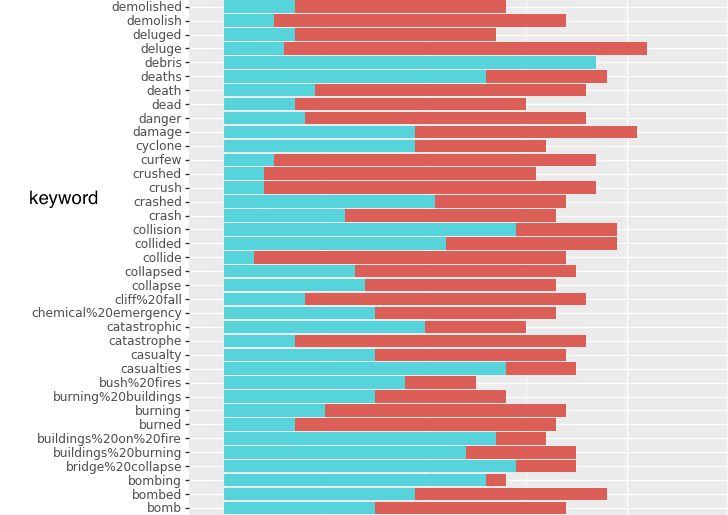
\includegraphics[scale=0.5]{keywords-vs-target.png}
  \caption{}
  \label{fig:keywords-vs-target}
\end{figure}

\begin{figure}[h!]
  \centering
  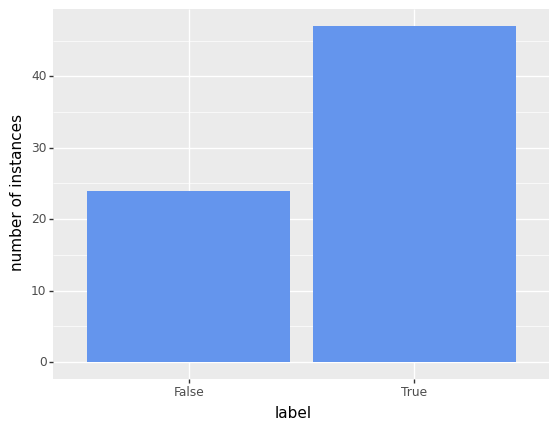
\includegraphics[scale=0.5]{mentioned-news.png}
  \caption{}
  \label{fig:mentioned-news}
\end{figure}

\begin{figure}[h!]
  \centering
  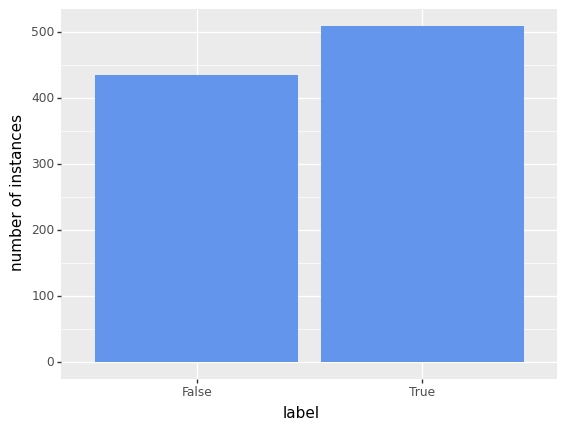
\includegraphics[scale=0.5]{contains-l1.png}
  \caption{}
  \label{fig:contains-l1}
\end{figure}

\begin{figure}[h!]
  \centering
  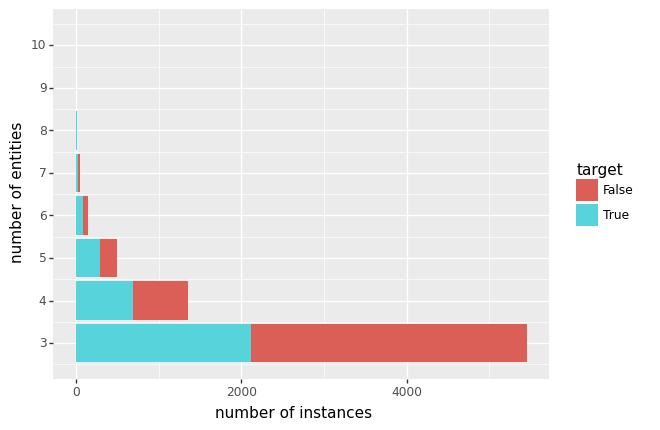
\includegraphics[scale=0.5]{num-ents-vs-target.png}
  \caption{}
  \label{fig:num-ents-vs-target}
\end{figure}


\begin{figure}[h!]
  \centering
  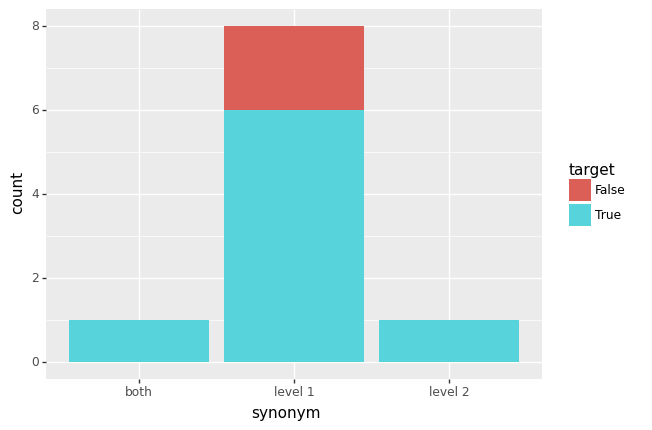
\includegraphics[scale=0.5]{hashtags-contain-synonyms.png}
  \caption{}
  \label{fig:hashtags-contain-synonyms}
\end{figure}

\begin{figure}[h!]
     \centering
     \begin{subfigure}[b]{0.42\textwidth}
         \centering
         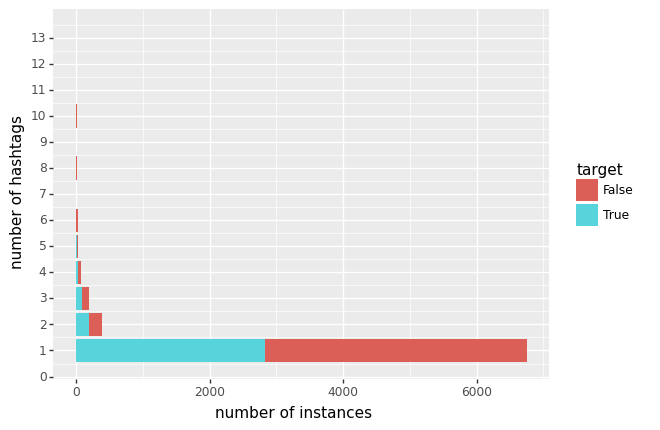
\includegraphics[width=\textwidth]{num-hashtags-vs-target.png}
         \caption{}
         \label{fig:num-hashtags-vs-target}
     \end{subfigure}
     \begin{subfigure}[b]{0.42\textwidth}
         \centering
         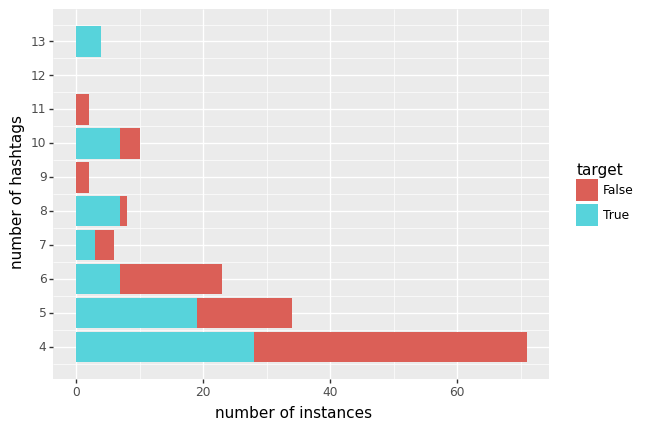
\includegraphics[width=\textwidth]{num-hashtags-vs-target-zoomed.png}
         \caption{}
         \label{fig:num-hashtags-vs-target-zoomed}
     \end{subfigure}
        \caption{}
        \label{fig:num-hashtags-graphs}
\end{figure}

\begin{figure}[h!]
     \centering
     \begin{subfigure}[b]{0.42\textwidth}
         \centering
         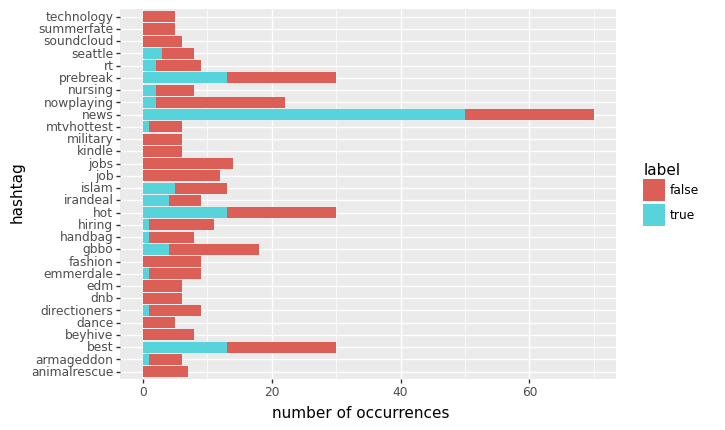
\includegraphics[width=\textwidth]{top-30-hashtags-false.png}
         \caption{}
         \label{fig:top-30-hashtags-false}
     \end{subfigure}
     \begin{subfigure}[b]{0.42\textwidth}
         \centering
         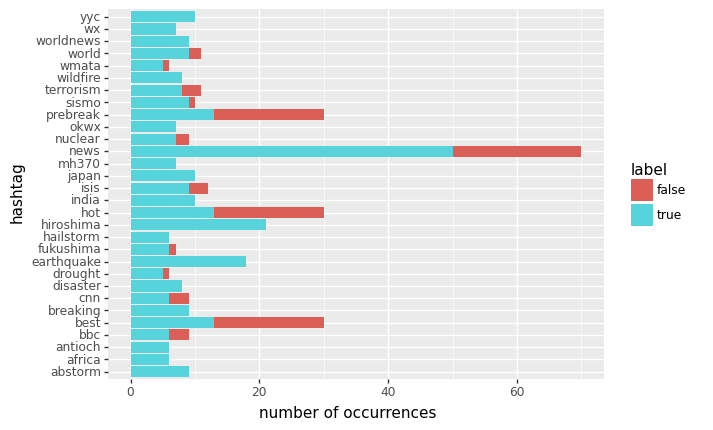
\includegraphics[width=\textwidth]{top-30-hashtags-true.png}
         \caption{}
         \label{fig:top-30-hashtags-true}
     \end{subfigure}
        \caption{}
        \label{fig:top-30-hashtags-graphs}
\end{figure}

\begin{table}[h]
  \centering
  \begin{tabular}{| l | p{0.4 \linewidth}|}
    \hline
    \textbf{Feature} & \textbf{Percentage of total instances with a value for the feature} \\ \hline
    Contains keyword & 100\% \\ \hline
    Contains location & 66.92\% \\ \hline
    Contains hashtag & 22.44\% \\ \hline
    Contains hashtag with level 1 synonym of "disaster" & 0.12\% \\ \hline
    Contains hashtag with level 2 synonym of "disaster" & 0.03\% \\ \hline
    Contains subject & 52.9\% \\ \hline
    Contains verb & 79.23\% \\ \hline
    Contains object & 79.39 \\ \hline
    Text contains level 1 synonym of "disaster" & 12.58\% \\ \hline
    Text contains level 2 synonym of "disaster" & 5.1\% \\ \hline
    Text contains words relating to damage  & 8.0\% \\ \hline
    News organisation mentioned & 0.95\% \\ \hline
    Relief organisation mentioned & 0.04\% \\ \hline
    Contains mentions & 25.4\% \\ \hline
    Contains one or more organisations & 59.72\% \\ \hline
    Contains one or more geopolitical entities & 15.19\% \\ \hline
    Contains one or more facilities & 1.73\% \\ \hline
  \end{tabular}
  \caption{}
  \label{tab:feature-stats}
\end{table}


\begin{figure}[h]
  \centering
  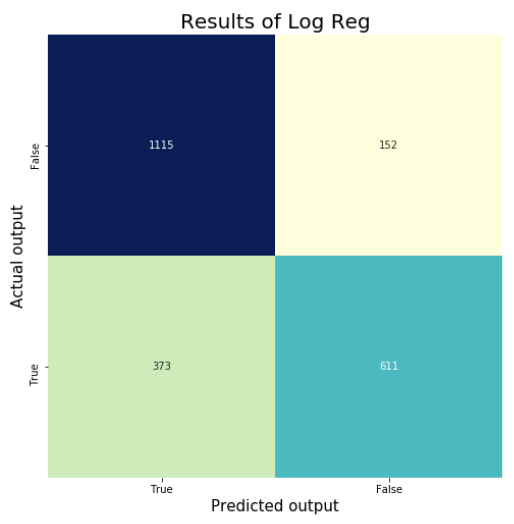
\includegraphics[scale=0.5]{confusion-matrix.png}
  \caption{Confusion matrix of 30\% of the tweets}
  \label{fig:confusion-matrix}
\end{figure}

\begin{figure}[h]
  \centering
  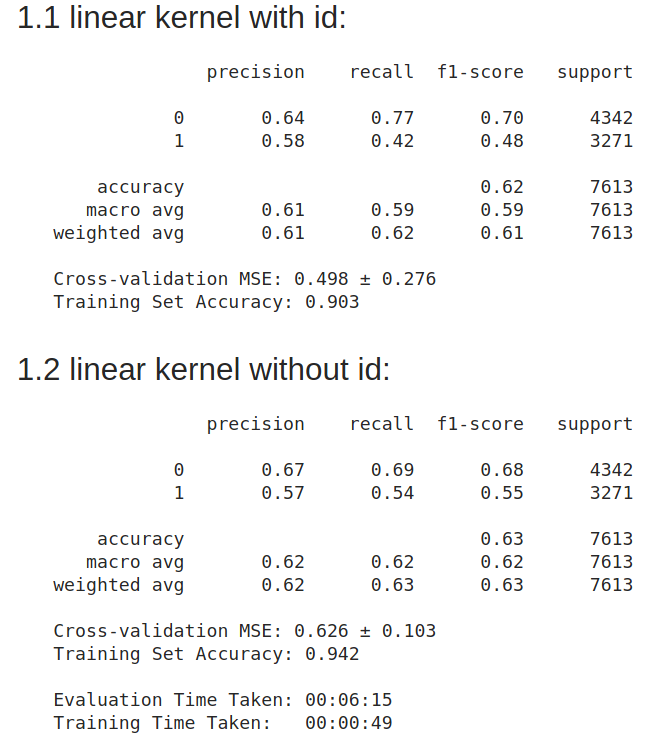
\includegraphics[scale=0.5]{feature-pre-elim-metrics.png}
  \caption{}
  \label{fig:feature-pre-elim-metrics}
\end{figure}

\begin{figure}[h]
  \centering
  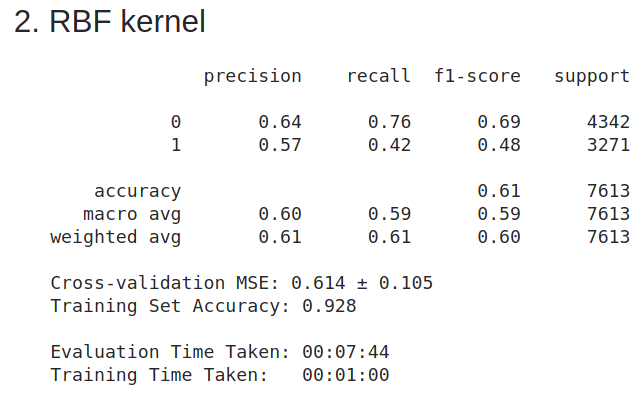
\includegraphics[scale=0.5]{rbf-kernel-tricks.png}
  \caption{}
  \label{fig:rbf-kernel-tricks}
\end{figure}

\begin{figure}[h]
  \centering
  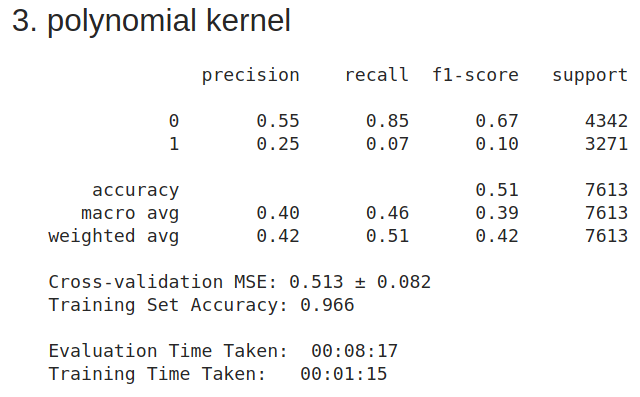
\includegraphics[scale=0.5]{poly-kernel-tricks.png}
  \caption{}
  \label{fig:poly-kernel-tricks}
\end{figure}

\begin{figure}[h]
  \centering
  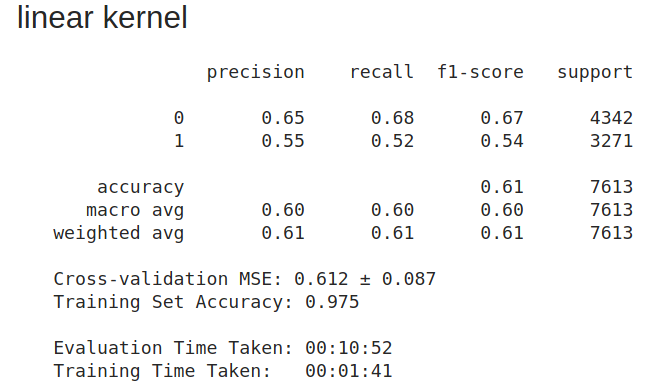
\includegraphics[scale=0.5]{linear-kernel-svc.png}
  \caption{}
  \label{fig:linear-kernel-svc}
\end{figure}

\begin{figure}[h]
  \centering
  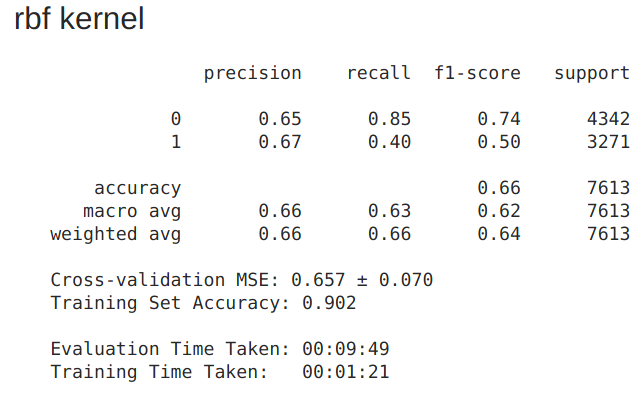
\includegraphics[scale=0.5]{rbf-kernel-svc.png}
  \caption{}
  \label{fig:rbf-kernel-svc}
\end{figure}

\begin{figure}[h]
  \centering
  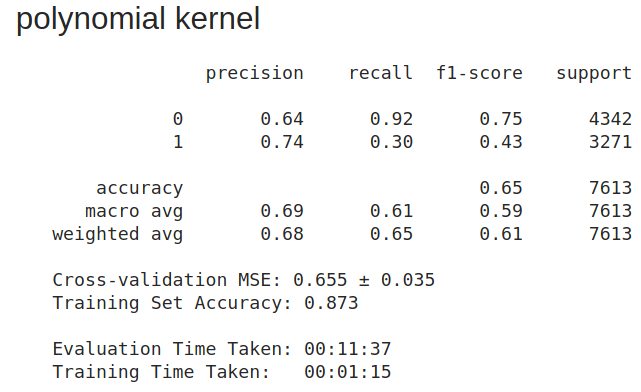
\includegraphics[scale=0.5]{poly-kernel-svc.png}
  \caption{}
  \label{fig:poly-kernel-svc}
\end{figure}

\begin{figure}[h]
  \centering
  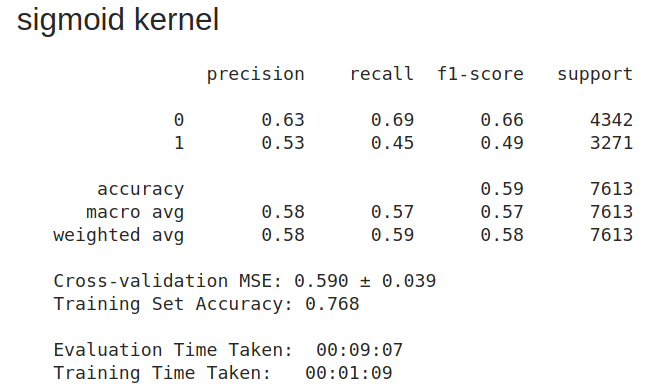
\includegraphics[scale=0.5]{sigmoid-kernel-svc.png}
  \caption{}
  \label{fig:sigmoid-kernel-svc}
\end{figure}

\begin{figure}[h]
  \centering
  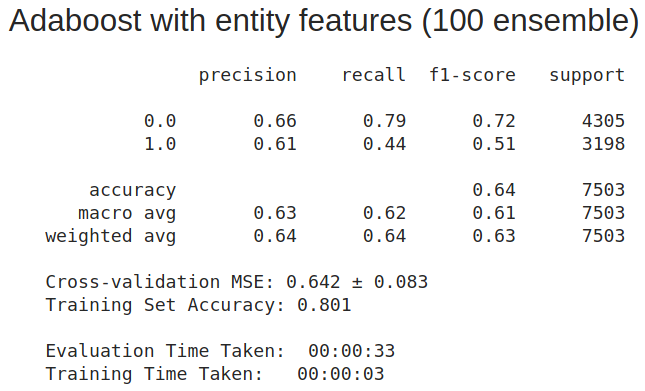
\includegraphics[scale=0.5]{adaboost.png}
  \caption{}
  \label{fig:adaboost}
\end{figure}

\begin{figure}[h]
  \centering
  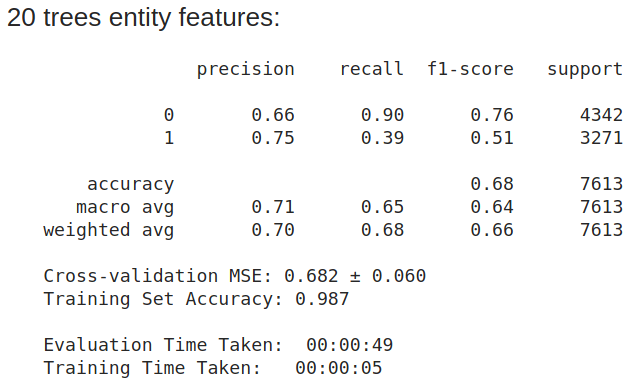
\includegraphics[scale=0.5]{20-trees.png}
  \caption{}
  \label{fig:20-trees}
\end{figure}

\begin{figure}[h]
  \centering
  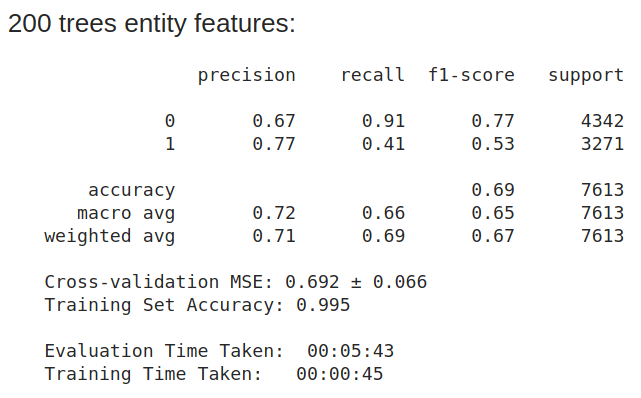
\includegraphics[scale=0.5]{200-trees.png}
  \caption{caption}
  \label{fig:200-trees}
\end{figure}

\begin{figure}[h]
  \centering
  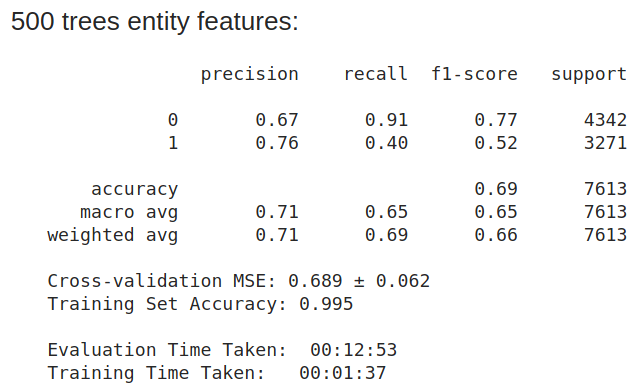
\includegraphics[scale=0.5]{500-trees.png}
  \caption{}
  \label{fig:500-trees}
\end{figure}

\begin{figure}[h]
  \centering
  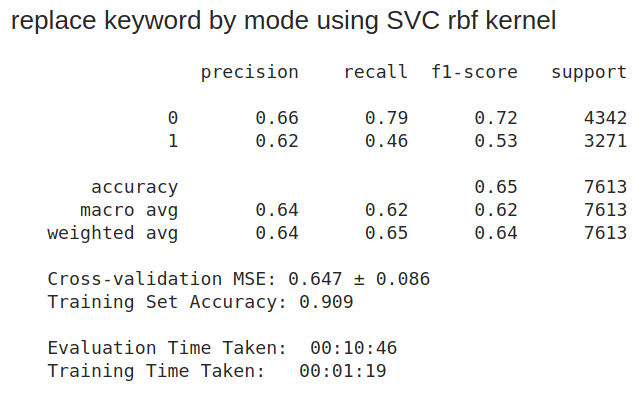
\includegraphics[scale=0.5]{replace-keyword-svc.png}
  \caption{}
  \label{fig:replace-keyword-svc}
\end{figure}

\begin{figure}[h]
  \centering
  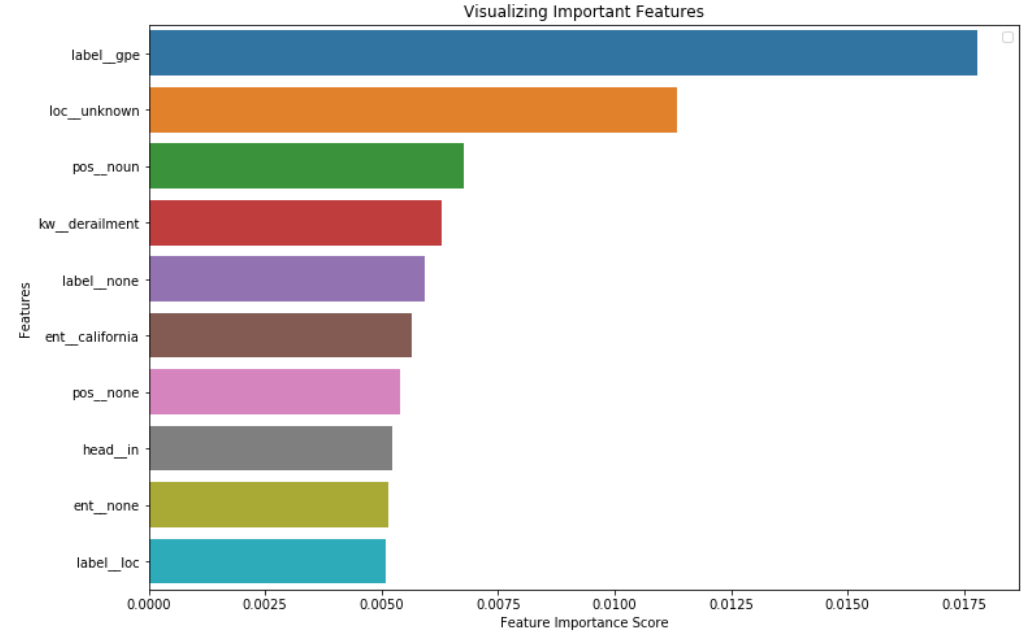
\includegraphics[scale=0.5]{top10-features-without-text.png}
  \caption{}
  \label{fig:top10-features-without-text}
\end{figure}

\begin{figure}[h]
  \centering
  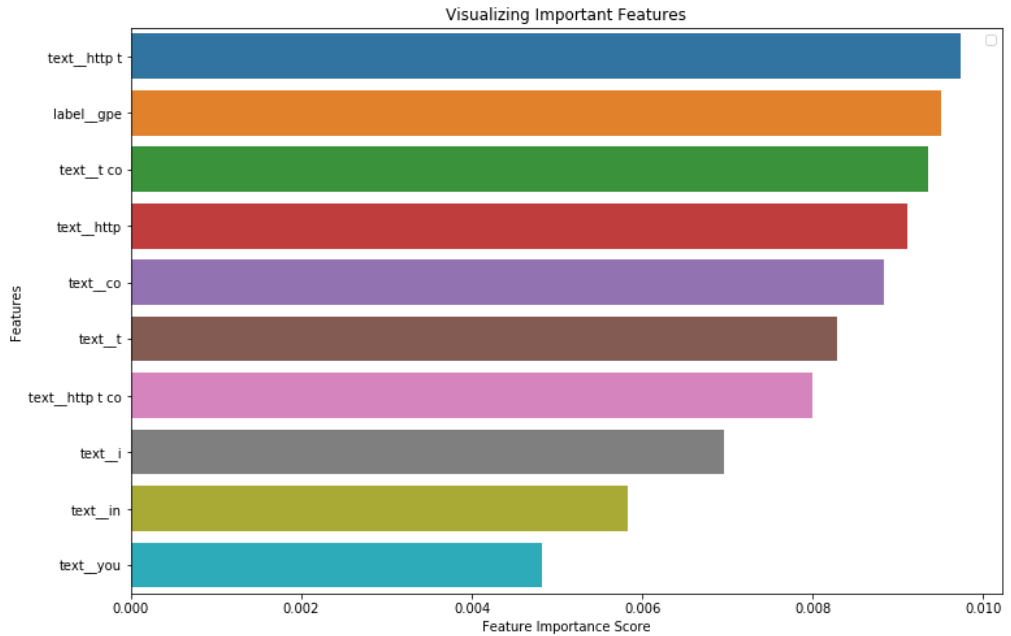
\includegraphics[scale=0.5]{important-features.png}
  \caption{}
  \label{fig:important-features}
\end{figure}

\begin{figure}[h]
  \centering
  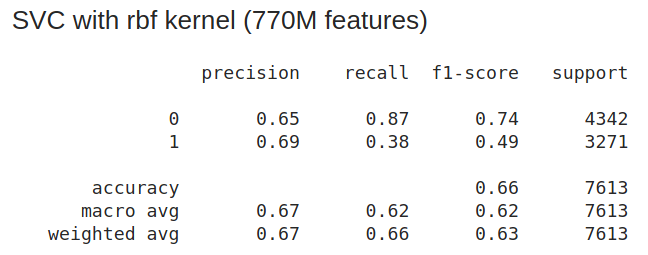
\includegraphics[scale=0.5]{svc-rbf-kernel.png}
  \caption{}
  \label{fig:svc-rbf-kernel}
\end{figure}

\begin{figure}[h]
  \centering
  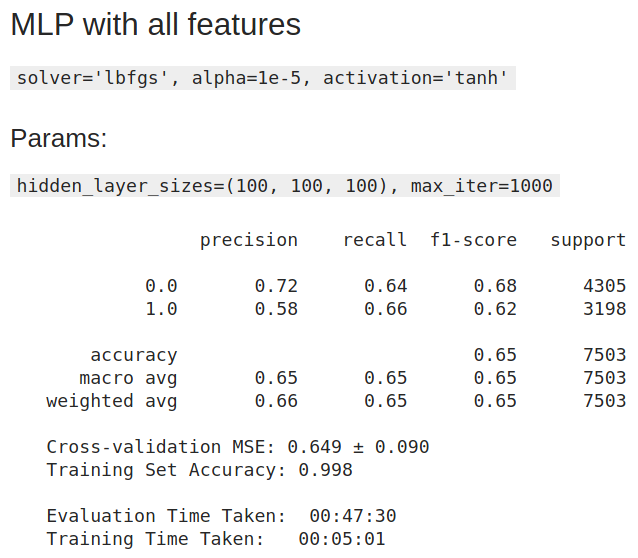
\includegraphics[scale=0.5]{mlp-all-features.png}
  \caption{}
  \label{fig:mlp-all-features}
\end{figure}

\begin{figure}[h]
  \centering
  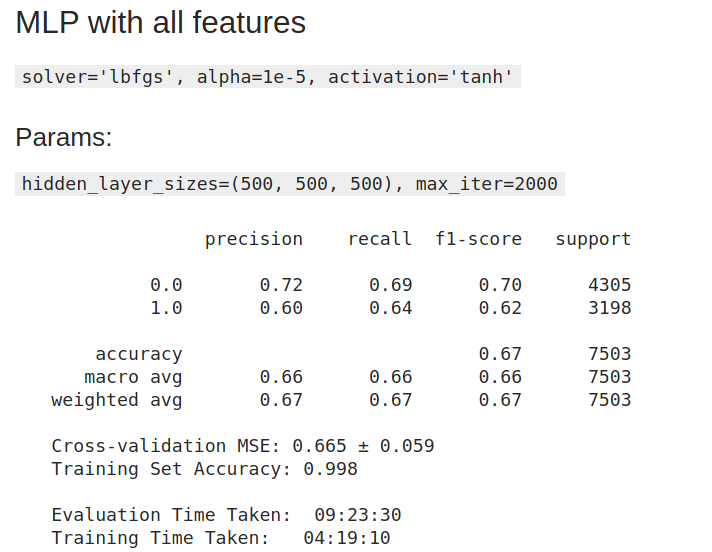
\includegraphics[scale=0.5]{mlp-all-features-2000.png}
  \caption{}
  \label{fig:mlp-all-features-2000}
\end{figure}

\begin{figure}[h]
  \centering
  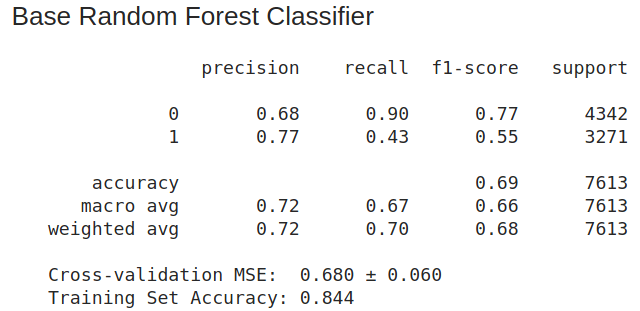
\includegraphics[scale=0.5]{base-random.png}
  \caption{}
  \label{fig:base-random}
\end{figure}

\begin{figure}[h]
  \centering
  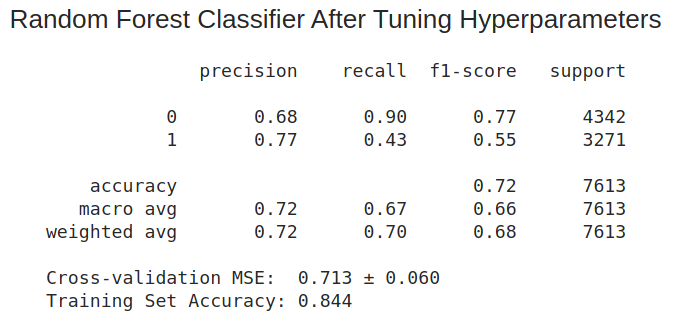
\includegraphics[scale=0.5]{random-hyper.png}
  \caption{}
  \label{fig:random-hyper}
\end{figure}
